\documentclass[hidelinks]{article}

\title{Numerical Methods for \\ High Performance Computing}
\author{Lorenzo Schiavone}
\date{\today}
\usepackage{graphicx}
\usepackage{hyperref}
\usepackage[utf8]{inputenc}
\usepackage{amsmath, amssymb, amsthm, mathtools, mathrsfs}
\usepackage[margin=1in]{geometry}

\usepackage[shortlabels]{enumitem}
\usepackage[colorinlistoftodos]{todonotes}
\usepackage{listings}
\usepackage{matlab-prettifier}
\usepackage{color}
\usepackage{subcaption}
\usepackage{caption}
\usepackage{float} 
\usepackage{comment}

\usepackage{graphics}
\usepackage{multicol}

\usepackage{tikz-3dplot}


\theoremstyle{definition}
\newtheorem{ex}{Exercise}

\usepackage{algorithm, algorithmicx}
\usepackage{algpseudocode}

\usepackage{array}
\usepackage{booktabs}

\lstset{
  language=C,
  basicstyle=\ttfamily\small,
  keywordstyle=\color{blue}\bfseries,
  stringstyle=\color{green!60!black},
  commentstyle=\color{gray}\itshape,
}
\DeclareMathOperator{\divg}{div}

\begin{document}
\maketitle
\tableofcontents

\pagebreak

\section{Problem Statement}
Consider the Transient Convection-Diffusion Equation 

\begin{equation}\tag{$D$}\label{eq:strong}
    \begin{aligned}
    \frac{\partial}{\partial t}u -K \Delta u + \divg(\beta u) &=0 && \text{in } \Omega, \\
    u(\mathbf{x}) &= 1 && \text{for } \mathbf{x} = \Gamma  \\
    \nabla u \cdot \nu &= 0 && \text{for } \mathbf{x}\in \partial\Omega \setminus \Gamma 
\end{aligned}
\end{equation}
for $\Omega = [0,1] \times [0,1]\times [0,1]$, $\Gamma = \{0\} \times \{0\} \times [0, .3]$, where $u=u(x,y,z)$ represents the scalar concentration of a solute dissolved in a fluid moving with velocity $\beta$ constant and homogenous and $K=\texttt{diag}(K_1,K_2,K_3)$ is the diffusion matrix assumed constant as well.

\begin{figure}[H]
\begin{center}
\tdplotsetmaincoords{75}{15}
\begin{tikzpicture}[tdplot_main_coords, scale=2]

% Draw cube edges
\draw[thick] (0,0,0) -- (1,0,0);  % x-axis edge
\draw[thick] (0,0,0) -- (0,1,0);  % y-axis edge
\draw[thick] (0,0,0) -- (0,0,1);  % z-axis edge

\draw[thick] (1,0,0) -- (1,1,0);
\draw[thick] (1,0,0) -- (1,0,1);

\draw[thick] (0,1,0) -- (1,1,0);
\draw[thick] (0,1,0) -- (0,1,1);

\draw[thick] (0,0,1) -- (1,0,1);
\draw[thick] (0,0,1) -- (0,1,1);

\draw[thick] (1,1,0) -- (1,1,1);
\draw[thick] (1,0,1) -- (1,1,1);
\draw[thick] (0,1,1) -- (1,1,1);

% Red dot at origin
\draw[thick, red] (0,0,0) -- (0,0,.3);
%\filldraw[red] (0,0,0) circle (1pt);         

\node[black] at (0.5, 0.5, 0.5) {$\Omega$};
\node[red] at (-0.15, 0, 0.15) {$\Gamma$};
\end{tikzpicture}
\end{center}
\caption{Domain of study.}
\end{figure}

\subsection{Weak Galerkin Formulation}
The Weak Formulation of (\ref{eq:strong}) is: find $u \in H^1(\Omega)$ such that boundary conditions hold and 

\begin{equation}\tag{$W$}\label{eq:weak}
\int_\Omega \frac{\partial u}{\partial t } v \,d\Omega + \int_\Omega K \nabla u \cdot \nabla v \,d\Omega + \int_\Omega \divg( \beta u) v\,d\Omega = 0
\end{equation}

for every $v \in H^1_0(\Omega)$, where we have integrated by part the first term and the boundary term vanishes because $v \in H^1_0(\Omega)$.

Now, considering the discretization $\mathcal{T}_h$ of $\Omega$ with nodes $\mathcal{N}_h = \{\mathbf{x}_1, \dots, \mathbf{x}_{n_\text{nodes}}\}$ and tetrahedral finite elements $\mathcal{E}_h$, we can approximate the function space $H^1(\Omega)$ with 
\[
\mathcal{V}_h = \text{span}\, \{\phi_1, \dots, \phi_{n_\text{nodes}} \}, 
\]
where the $\phi_i$ are the piecewise linear Lagrangian basis function. Then, we can write the approximate solution $u_h(t) = \sum_{j=0}^{n_\text{nodes}} u_j(t) \phi_j$ and, as $\mathcal{V}_h$ is a finite dimensional vector space, is enough to verify Equation (\ref{eq:weak}) for the basis functions $\phi_i$. It yields the Weak Galerkin Formulation: find $u_h(t) \in \mathcal{V}_h$ such that boundary conditions hold and

\begin{equation}\tag{$W_h$}\label{eq:weakGalerkin1}
\int_\Omega \sum_{j=1}^{n_\text{nodes}} u'_j(t)\phi_j\phi_i \,d\Omega +\int_\Omega \sum_{j=1}^{n_\text{nodes}} u_j(t) K \nabla \phi_j \cdot \nabla \phi_i \,d\Omega + \int_\Omega \sum_{j=1}^{n_\text{nodes}} u_j(t) \divg( \beta \phi_j) \phi_i\,d\Omega = 0
\end{equation}

or 

\begin{equation}\tag{$W_h$}\label{eq:weakGalerkin2}
\sum_{j=1}^{n_\text{nodes}} u'_j(t) \left( \int_\Omega \phi_j\phi_i \,d\Omega \right) + \sum_{j=1}^{n_\text{nodes}} u_j(t) \left(\int_\Omega K  \nabla \phi_j \cdot \nabla \phi_i \,d\Omega\right) + \sum_{j=1}^{n_\text{nodes}} u_j(t) \left(\int_\Omega  \divg( \beta \phi_j) \phi_i\,d\Omega\right) = 0
\end{equation}

that in matrix form reads \[ P\mathbf{u}' + H\mathbf{u} + B\mathbf{u} = 0\] where $\mathbf{u} = (u_1, \dots, u_{n_\text{nodes}})^T$, and the mass matrix $P$, the diffusion stiffness matrix $H$ and the non-symmetric convective matrix $B$ have components, respectively,
\[P_{ij} = \int_\Omega \phi_j \phi_i\, d\Omega ,\quad\quad H_{ij} = \int_\Omega K \nabla \phi_j \cdot \nabla \phi_i\, d\Omega \quad \text{and} \quad B_{ij} = \int_\Omega  \divg( \beta \phi_j) \phi_i\,d\Omega.\]

\subsection{Finite Elements Matrices}

Inside each tetrahedral element $e\in\mathcal{E}$ with vertices $\mathbf{x}_i, \mathbf{x}_j, \mathbf{x}_k, \mathbf{x}_m$ only the corresponding basis function $\phi_i,\phi_j,\phi_k,\phi_m$ are non zero. Their local expression is 
\[
\phi_l^{(e)} (x,y,z)= \frac{a_l + b_l x + c_l y + d_l z}{6V^{(e)}} \quad \text{for } l \in \{i,j,k,m\},
\]
where $V^{(e)}$ is the surface measure of the element,
\[
V^{(e)} = \frac{1}{6}\det \left(\begin{bmatrix}
    1 & x_i & y_i & z_i \\ 1 & x_j & y_j & z_j\\ 1 & x_k & y_k & z_k \\ 1 & x_m & y_m & z_m
\end{bmatrix} \right),
\]
and the coefficients $\mathbf{a}, \mathbf{b}, \mathbf{c}, \mathbf{d}$ are computed so that $\phi_l(\mathbf{x_r}) = \delta_{lr}$, i.e., 

\begin{align*}
a_i &= \det \begin{bmatrix} x_j & y_j & z_j \\ x_k & y_k & z_k \\ x_m & y_m & z_m \end{bmatrix}& b_i &= - \det \begin{bmatrix} 1 & y_j & z_j \\ 1 & y_k & z_k \\ 1 & y_m & z_m \end{bmatrix} & & & a_j &= - \det \begin{bmatrix} x_i & y_i & z_i \\ x_k & y_k & z_k \\ x_m & y_m & z_m \end{bmatrix}& b_j &= \det \begin{bmatrix} 1 & y_i & z_i \\ 1 & y_k & z_k \\ 1 & y_m & z_m \end{bmatrix}\\
c_i &= \det \begin{bmatrix} 1 & x_j & z_j \\ 1 & x_k & z_k \\ 1 & x_m & z_m \end{bmatrix} & d_i &= - \det \begin{bmatrix} 1 & x_j & y_j \\ 1 & x_k & y_k \\ 1 & x_m & y_m \end{bmatrix}      & & & c_j &= - \det \begin{bmatrix} 1 & x_i & z_i \\ 1 & x_k & z_k \\ 1 & x_m & z_m \end{bmatrix}& d_j &= \det \begin{bmatrix} 1 & x_i & y_i \\ 1 & x_k & y_k \\ 1 & x_m & y_m \end{bmatrix}\\ \\
a_k &= \det \begin{bmatrix} x_i & y_i & z_i \\ x_j & y_j & z_j \\ x_m & y_m & z_m \end{bmatrix}& b_k &= - \det \begin{bmatrix} 1 & y_i & z_i \\ 1 & y_j & z_j \\ 1 & y_m & z_m\end{bmatrix}& & & a_m &= - \det \begin{bmatrix} x_i & y_i & z_i \\ x_j & y_j & z_j \\ x_k & y_k & z_k \end{bmatrix}& b_m &= \det \begin{bmatrix} 1 & y_i & z_i \\ 1 & y_j & z_j \\ 1 & y_k & z_k\end{bmatrix} \\
c_k &= \det \begin{bmatrix} 1 & x_i & z_i \\ 1 & x_j & z_j \\ 1 & x_m & z_m \end{bmatrix}& d_k &= - \det \begin{bmatrix} 1 & x_i & y_i \\ 1 & x_j & y_j \\ 1 & x_m & y_m \end{bmatrix}     & & & c_m &= - \det \begin{bmatrix} 1 & x_i & z_i \\ 1 & x_j & z_j \\ 1 & x_k & z_k \end{bmatrix}& d_m &=\det \begin{bmatrix} 1 & x_i & y_i \\ 1 & x_j & y_j \\ 1 & x_k & y_k \end{bmatrix}\\
\end{align*}
Then, \[\nabla \phi_i^{(e)} = \frac{1}{6V^{(e)}}\begin{bmatrix}
    b_i \\ c_i \\ d_i
\end{bmatrix} \] is constant and the local diffusion stiffness matrix is 
\begin{align*}
H_{ij}^{(e)} &= \int_e K \frac{1}{6V^{(e)}}(b_i, c_i, d_i)^T \cdot \frac{1}{6V^{(e)}}(b_j, c_j, d_j)^T \,d\Omega \\ &= \frac{|V^{(e)}|}{{36V^{(e)}}^2} (K_1b_ib_j + K_2c_ic_j + K_3d_id_j) = \frac{1}{36|V^{(e)}|} (K_1b_ib_j + K_2c_ic_j + K_3d_id_j).
\end{align*}
Compactly, if we collect $\mathbf{b} = \begin{bmatrix} b_i & b_j & b_k & b_m\end{bmatrix}$ and, likewise $\mathbf{c} = \begin{bmatrix} c_i & c_j & c_k & c_m\end{bmatrix}$ and $\mathbf{d} = \begin{bmatrix} d_i & d_j & d_k & d_m \end{bmatrix}$, we can write 
\[ H^{(e)} = \frac{1}{36|V^{(e)}|}(K_1\mathbf{b}^T\mathbf{b} + K_2\mathbf{c}^T\mathbf{c} +  K_3\mathbf{d}^T\mathbf{d}).
\]
\paragraph{Convective Matrix}
Moreover, since \[
\divg (\beta \phi_j) = \beta \cdot \nabla \phi_j = \frac{1}{6V^{(e)}}\left(\beta \cdot \begin{bmatrix}
    \mathbf{b} \\
    \mathbf{c} \\
    \mathbf{d}
\end{bmatrix} \right)_j =: \frac{1}{6V^{(e)}} \sigma_j,
\] 
where $\sigma$ is the row vector $\beta \cdot \begin{bmatrix}
    \mathbf{b} \\
    \mathbf{c} \\
    \mathbf{d}
\end{bmatrix}$ for brevity, and
\[
\int_e \phi^{(e)}_i \, d\Omega = \frac{1}{4} |V^{(e)}| \quad \text{as} \quad \phi^{(e)}_i + \phi^{(e)}_j + \phi^{(e)}_k + \phi^{(e)}_m= 1,
\]
we have that the local convective matrix is
\[
B_{ij}^{(e)} = \int_e \divg (\beta \phi^{(e)}_j) \phi^{(e)}_i \, d\Omega = \frac{1}{6V^{(e)}}\sigma_j \int_e \phi^{(e)}_i \, d\Omega = \frac{1}{6V^{(e)}}\sigma_j \frac{1}{4} V^{(e)} = \frac{\text{sgn}\, V^{(e)}}{24} \sigma_j.
\]
In matrix form,
\[
B^{(e)} = \frac{\text{sgn}\, V^{(e)}}{24} \begin{bmatrix} \sigma \\ \sigma \\ \sigma \\ \sigma
\end{bmatrix},
\]
where the rows are equal as the coefficients are independent of the row index.

\paragraph{Mass Matrix} 
The mass matrix coefficients are
\[
P^{(e)}_{ij} = \int_\Omega\phi^{(e)}_i\phi^{(e)}_j\,d\Omega,
\]
that in matrix form is
\[
P^{(e)} = \frac{|V^{(e)}|}{20}\begin{bmatrix}
    2 & 1 & 1 & 1 \\ 1 & 2 & 1 & 1 \\ 1 & 1 & 2 & 1 \\ 1 & 1 & 1 & 2
\end{bmatrix}.
\]  

\section{Matrix CSR format}
Matrices are stored in Compressed Sparse Row (CSR) format for memory efficiency. Each matrix $N\times N$ is described by:
\begin{itemize}
    \item a vector of double \texttt{coef} with the non zero coefficients,
    \item a vector of int \texttt{ja} with the same length of \texttt{coef} where each component is the column index of the corresponding non zero coefficient,
    \item a vector of int \texttt{iat} of dimension $N+1$ where $\texttt{iat}(i)$ has the index where the coefficients of the row $i$ begin in \texttt{coef}.
\end{itemize}

Using this structure, the matrix vector product $A v = b$ is computed as in the following snippet, where $N$ is the dimension of $A$.

\begin{lstlisting}
    for(int i = 0; i < N; i++){
        double sum = 0.0;
        for(int k = iat[i]; k < iat[i+1]; k++)
            sum += coef[k] * v[ja[k]];
        b[i] = sum;
    }
\end{lstlisting}

\section{Parallel Assembly}

Given the tetrahedral discretization of the unit cube, e.g., ``Cubo\_4820.coor'' for the node coordinates and ``Cubo\_4820.tetra'' for the mesh connectivities, the topology of the sparse matrices $P$, $H$, and $B$, i.e., the vectors \texttt{iat} and \texttt{ja}, is computed using a routine in \texttt{topol.cpp}, a file already provided.
For parallelization, we used \emph{OpenMP} directives in C, experimenting with two methods.

\paragraph{Methods}
In the first method, we open a parallel region within the main loop over the elements. When adding local contributions to the global matrices, we avoid data races using the \emph{omp atomic} directive, which ensures safe access to specific memory locations.
In the second method, we divide the nodes among threads, and each thread is responsible for assembling only the rows corresponding to the nodes assigned to it. To accomplish this, we open a parallel region before the main loop, and each thread iterates through all elements. At the beginning of each loop iteration, we check whether any node of the current element lies within the index range handled by the thread. If none do, the thread skips the element; otherwise, it proceeds with the assembly.

\paragraph{RCM Ordering}
The RCM Ordering minimize the maximum distance from the diagonal of the connectivity matrix as we can see in Figure \ref{fig:rcm}. This ordering well suited for the second method, so that most of the elements have all the nodes dealt by the same thread and very few are shared between threads avoid repeating the computation of local matrices different times.

\begin{figure}[H]
    \centering
    \begin{subfigure}{.45\textwidth}
        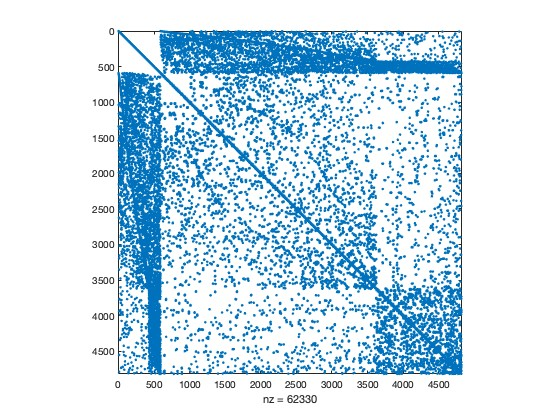
\includegraphics[width = \textwidth]{pic/topol4820_native.jpg}
    \end{subfigure} \hfill
    \begin{subfigure}{.45\textwidth}
        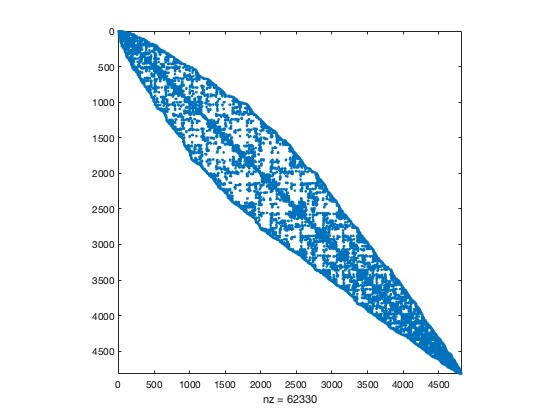
\includegraphics[width = \textwidth]{pic/topol4820_rcm.jpg}
    \end{subfigure} 
    \caption{Comparison between the Sparsity Pattern of the Native Order, in the left, and RCM Order, in the right, for Cubo\_4820.}\label{fig:rcm}
\end{figure}

\subsection{Parallelisation Improvements}
\paragraph{Time}
For the mesh with 1772481 nodes (Cube\_1772481) we record in Table \ref{tab:assemblytimes} the total wallclock time for the assembly using the two different methods and orders.
% In Tables \ref{tab:first} and \ref{tab:second} are recorded the wallclock time for the assembly using different mesh size and method. 

\begin{table}[H]
    \centering
    \begin{tabular}{| c | c c | c c | }
        \hline 
        np & \multicolumn{2}{c|}{Native Order} & \multicolumn{2}{c|}{RCM Order} \\ \hline
        method & 1 & 2 		& 1 & 2 		\\ \hline
        1 & 8.219900 & 5.204082 & 8.249664 & 5.618524   \\ 
        2 & 4.630122 & 3.205535 & 4.689079 & 3.162474   \\
        3 & 4.060645 & 2.878401 & 4.205213 & 2.737441   \\
        4 & 3.634686 & 2.751820 & 3.705338 & 2.398958   \\ \hline

    \end{tabular}
    \caption{Wallclock time for the assembly of Cube\_1772481 per number of threads using the different methods.}\label{tab:assemblytimes}
\end{table}

\paragraph{Speedup} We compute the speedup as $S_p = T_1 / T_p$ and obtain the following values.

\begin{table}[H]
    \centering
    \begin{tabular}{| c c  | c c | c c | }
        \hline 
        np & \multicolumn{2}{c|}{Native Order} & \multicolumn{2}{c|}{RCM Order} \\ \hline
        & method & 1 & 2 		& 1 & 2 		\\ \hline
        1 && 8.219900 & 5.204082 & 8.249664 & 5.618524   \\ 
        2 && 4.630122 & 3.205535 & 4.689079 & 3.162474   \\
        3 && 4.060645 & 2.878401 & 4.205213 & 2.737441   \\
        4 && 3.634686 & 2.751820 & 3.705338 & 2.398958   \\ \hline

    \end{tabular}
    \caption{Speedup for the assembly of Cube\_1772481 per number of threads using the different methods.}\label{tab:assemblyspeedups}
\end{table}

% \begin{table}[H]
%     \centering
%     \begin{tabular}{|l|cccc|cccc|}
%         \hline 
%         mesh     & \multicolumn{4}{c|}{Native Orders}            & \multicolumn{4}{c|}{RCM Orders}   \\ \hline
%         np       & 1 & 2 & 3 & 4                                 & 1 & 2 & 3 & 4                     \\ \hline
%         591      & 0.003498 & 0.002196 & 0.001492 & 0.001343     & 0.002204 & 0.001836 & 0.001522 & 0.001348  \\
%         4820     & 0.029394 & 0.016465 & 0.017465 & 0.016776     & 0.033074 & 0.026714 & 0.017348 & 0.016971  \\
%         35199    & 0.139041 & 0.084434 & 0.078921 & 0.074565     & 0.146572 & 0.104031 & 0.083276 & 0.073265  \\
%         246389   & 1.083549 & 0.660812 & 0.622493 & 0.454520     & 1.087817 & 0.578902 & 0.527128 & 0.463474  \\
%         1772481  & 8.674350 & 5.024438 & 4.384249 & 3.763095     & 8.235272 & 5.036050 & 4.239713 & 3.669412  \\ \hline
%     \end{tabular}
%     \caption{Wallclock time per mesh per number of processors using the first method.}\label{tab:first}
% \end{table}

% \begin{table}[H]
%     \centering

%     \begin{tabular}{|l|cccc|cccc|}
%         \hline
%         mesh     & \multicolumn{4}{c|}{Native Orders}           & \multicolumn{4}{c|}{RCM Orders}   \\ \hline
%         np       & 1 & 2 & 3 & 4                                & 1        & 2        & 3        & 4                     \\ \hline
%         591      & 0.001416 & 0.001367 & 0.001582 & 0.001504    & 0.001735 & 0.001542 & 0.001306 & 0.001068              \\
%         4820     & 0.016920 & 0.008194 & 0.013895 & 0.010358    & 0.016194 & 0.008159 & 0.011808 & 0.012608              \\
%         35199    & 0.107847 & 0.070413 & 0.066152 & 0.063732    & 0.102554 & 0.065730 & 0.053469 & 0.058253              \\
%         246389   & 0.726559 & 0.432734 & 0.404094 & 0.380202    & 0.777682 & 0.423994 & 0.374354 & 0.335085              \\
%         1772481  & 5.563172 & 3.334491 & 3.119737 & 2.856767    & 5.565595 & 3.227776 & 2.997635 & 2.711643              \\ \hline
%     \end{tabular}
%     \caption{Wallclock time per mesh per number of processors using the second method.}\label{tab:second}
% \end{table}

We can notice that the second method generally reduces the wallclock time by completely avoiding the atomic clause. 
For showing the improvements obtained with the parallelization, we only consider the larger instances, i.e., 246389 and 1772481, as for smaller the parallelization cannot be fully exploited and the overheads are counterproductive.

\section{GMRES}

The Generalized Minimal Residual method (GMRES) is an iterative Krylov subspace method used to solve nonsymmetric and possibly indefinite systems of linear equations of the form
\[
Ax = b,
\]
where \( A \in \mathbb{R}^{n \times n} \) is a general (not necessarily symmetric) matrix, and \( b \in \mathbb{R}^n \) is the right-hand side vector.

GMRES constructs an approximate solution \( x_k \) in the Krylov subspace
\[
\mathcal{K}_k(A, r_0) = \text{span} \{ r_0, Ar_0, A^2r_0, \dots, A^{k-1}r_0 \},
\]
where \( r_0 = b - Ax_0 \) is the initial residual, such that the residual norm \( \| b - Ax_k \|_2 \) is minimized at each iteration \( k \).

The method builds an orthonormal basis of \( \mathcal{K}_k(A, r_0) \) using the Arnoldi process, resulting in a Hessenberg matrix \( H_k \). The approximate solution is then computed by solving a least-squares problem involving \( H_k \).

\subsection{Pseudocode of the GMRES Algorithm}

Below is a simplified version of the preconditoned GMRES algorithm:

\begin{algorithm}[H]
\caption{GMRES}
\begin{algorithmic}
\Require $A$, $M^{-1}$, rhs $b$, $x_0$, \texttt{maxit}, \texttt{tol}
\State \( r_0 = M^{-1}(b - Ax_0) \)
\State \( \beta = \|r_0\|_2 \), \( v_1 = r_0 / \beta \)
\For{$j = 1, 2, \dots, \texttt{maxit}$}
    \State Compute \( w = M^{-1}(Av_j) \)
    \For{$i = 1, \dots, j$}
        \State \( h_{i,j} = w^T v_i \)
        \State \( w = w - h_{i,j} v_i \)
    \EndFor
    \State \( h_{j+1,j} = \|w\|_2 \)
    \If{\( h_{j+1,j} = 0 \)} \Comment{happy breakdown}
        \State break
    \EndIf
    \State \( v_{j+1} = w / h_{j+1,j} \)
    \State Solve least squares problem \( \min \| \beta e_1 - H_j y \|_2 \)
    \State \( x_j = x_0 + V_j y \)
    \If{\( \| b - Ax_j \|_2 < \beta \cdot \texttt{tol} \)}
        \State \Return \( x_j \)
    \EndIf
\EndFor
\end{algorithmic}
\end{algorithm}

To solve the least squares problem, the QR factorization of the Hessenberg matrix $H_j$ is computed. Moreover, we have that $ \| b - Ax_j \|_2 = \min \| \beta e_1 - H_j y \|_2 \ = |(Q^Te_1)_{j+1}|$ and there is no need to solve explicitely the least square problem, that can be done once for all at the end.

\paragraph{Numerical Implementation of QR}
At first, we implement the full QR with the Modified Gram Schmidt method. Later, we exploit the incremental nature of the problem to update the QR factorization through Givens rotations. It allows to be more efficient both in memory and in computing resources.

At the step $j$ the QR factorization of the \((j+1) \times j\) upper Hessenberg matrix \( \widetilde{H}_j \) is
\[
\widetilde{Q}^T_j \widetilde{H}_j = \widetilde{R}_j,
\]
where \( \widetilde{Q}^T_j \in \mathbb{R}^{(j+1) \times (j+1)} \) is orthogonal and \( \widetilde{R}_j \in \mathbb{R}^{(j+1) \times j} \) is upper triangular. Because \( \widetilde{R}_j \) has one more row than columns, it can be written as
\[
\widetilde{R}_j = 
\begin{bmatrix}
R_j \\
0
\end{bmatrix},
\]
where \( R_j \in \mathbb{R}^{j \times j} \) is upper triangular.
At the next step, as the Hessenberg matrix is augmented only by one row and one column:
\[
\widetilde{H}_{j+1} = 
\begin{bmatrix}
\widetilde{H}_j & h_{j+1} \\
0 & h_{j+2,j+1}
\end{bmatrix},
\]
where \( h_{j+1} \in \mathbb{R}^{j+1} \) is the new column, to update the QR decomposition, we first extend \( Q^T_j \) by embedding it into a \((j+2) \times (j+2)\) identity matrix:
\[
\begin{bmatrix}
Q^T_j & 0 \\
0 & 1
\end{bmatrix} \widetilde{H}_{j+1} =
\begin{bmatrix}
R_j & r_{j+1} \\
0 & \rho \\
0 & \sigma
\end{bmatrix}.
\]
This matrix is almost upper triangular, except for the entry \( \sigma \). To eliminate \( \sigma \), we apply a Givens rotation
\[
G_j = 
\begin{bmatrix}
I_j & 0 & 0 \\
0 & c_j & s_j \\
0 & -s_j & c_j
\end{bmatrix},
\]
where the cosine and sine coefficients are defined as
\[
c_j = \frac{\rho}{\sqrt{\rho^2 + \sigma^2}}, \qquad
s_j = \frac{\sigma}{\sqrt{\rho^2 + \sigma^2}}.
\]
The new orthogonal matrix becomes
\[
Q^T_{j+1} = G_j 
\begin{bmatrix}
Q^T_j & 0 \\
0 & 1
\end{bmatrix},
\]
and the updated Hessenberg factorization satisfies
\[
Q^T_{j+1} \widetilde{H}_{j+1} =
\begin{bmatrix}
R_j & r_{j+1} \\
0 & r_{j+1,j+1} \\
0 & 0
\end{bmatrix},
\quad \text{with} \quad
r_{j+1,j+1} = \sqrt{\rho^2 + \sigma^2}.
\]
In addition, the new residual vector $\widetilde{Q}^T_{j+1}e_1$ is easily updated as well to be
\[
s_\text{new} = G_j s_\text{prev},
\]
from the previous residual vector $s_\text{prev}$.

\subsection{GMRES with Restarts}

One of the most computationally expensive aspects of the GMRES algorithm is the computation of scalar products involving large vectors. As the number of iterations increases, the cost of orthonormalizing the new vector $Av_n$ also grows, due to the expanding Krylov subspace.

A common strategy to mitigate this cost is to restart the algorithm after a fixed number of iterations. Specifically, once the Krylov basis reaches a predetermined maximum size, the algorithm is restarted using the current approximate solution as the new initial guess. This restart mechanism limits the size of the Krylov subspace and, consequently, the cost of orthonormalization and QR factorization. As a result, optimizing the QR decomposition becomes less critical, since the matrices involved remain relatively small—especially when compared to the size the Krylov basis would otherwise reach.

\section{Numerical Solution and SpeedUp}
We set $K_1 = 0.4$, $K_2 = 0.1$, $K_3 = 0.1$ and $\beta = \begin{bmatrix} 1 &1& 2 \end{bmatrix}$, so that we should see more diffusion in the $x$ direction and convection in $z$ direction. The result for the topology \emph{Cubo\_246389} is represented in Figure \ref{fig:numericalsol}.

\begin{figure}[H]
    \centering
    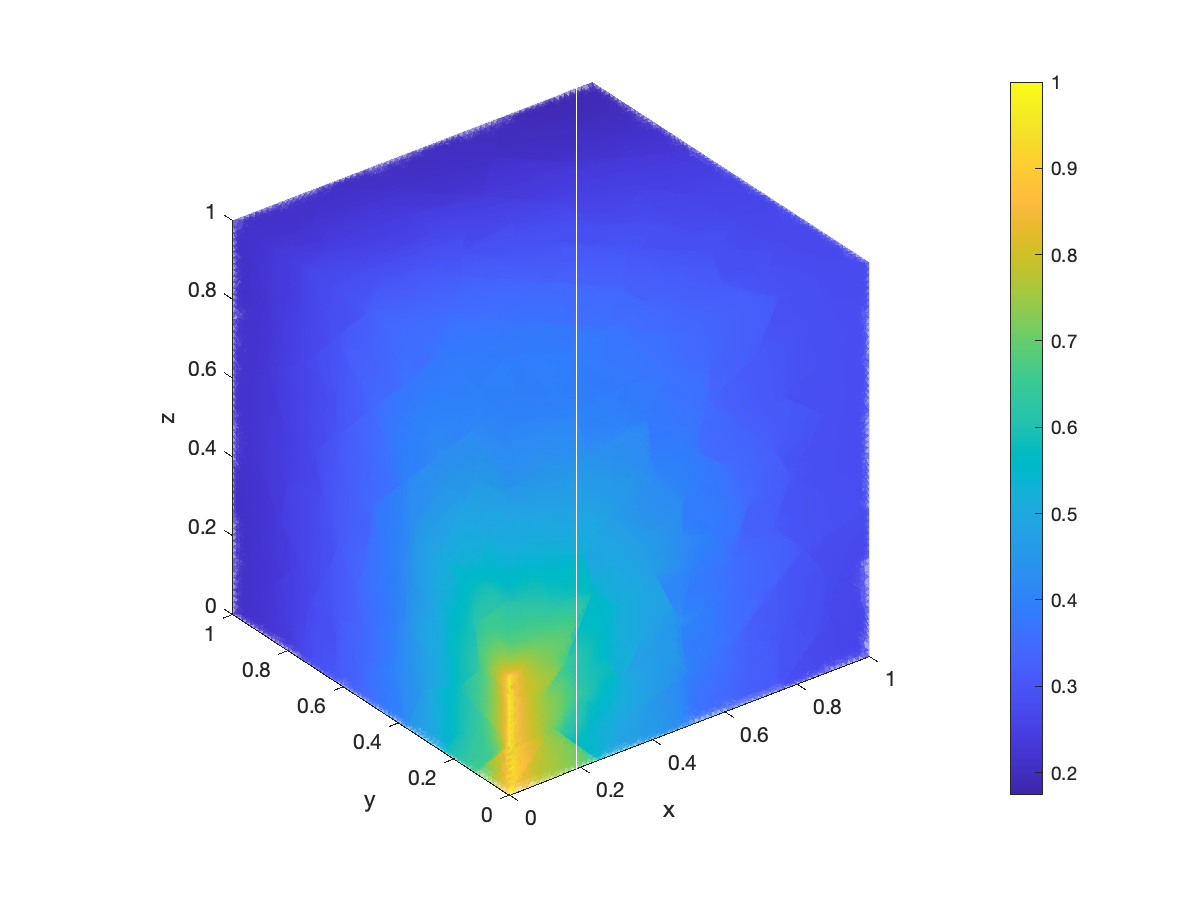
\includegraphics[width= 0.6\textwidth]{pic/sol246389.eps}
    \caption{Numerical Solution for \emph{Cubo\_246389}.}\label{fig:numericalsol} 
\end{figure}

\paragraph{SpeedUp}
We record the wallclock time for different runs of the gmres algorithm with different mesh resolution, with full QR or update QR with Givens rotations and with different number of threads.

Table \ref{tab:gmrestime} has the times for the GMRES algorithm without restart. As for finer mesh the problem gets worse conditioned, it requires more number of iterations and the computation of scalars product to orthogonormalize the new vector slow down and the Hessenberg matrix gets large enough to see a difference in performance between fullQR and updateQR with Givens rotations. For instance, for this particular equation, 692 iterations are needed for Cubo\_246389, 327 for Cubo\_35199 and 152 for Cubo\_2480.

\begin{table}[H]
    \centering
    \scalebox{0.85}{
    \begin{tabular}{|l|cccc|cccc|}
        \hline
        mesh     & \multicolumn{4}{c|}{Full QR}                         & \multicolumn{4}{c|}{Givens Rotations}                  \\ \hline
        np       & 1 & 2 & 3 & 4                                        & 1           & 2          & 3          & 4              \\ \hline
        591      & 0.018584 & 0.026168 & 0.021910 & 0.038606            & 0.016536    & 0.022566   & 0.020040   & 0.012172       \\
        4820     & 0.245137 & 0.219408 & 0.253363 & 0.365317            & 0.176397    & 0.157603   & 0.155172   & 0.114681       \\
        35199    & 6.691650 & 5.263159 & 5.521273 & 5.481706            & 3.850077    & 3.133227   & 2.558239   & 2.028428       \\
        246389   & 192.774403 & 172.514156 & 166.784374 & 165.938683    & 141.900566  & 118.400026 & 109.071518 & 108.034066     \\ \hline
        % 1772481  &  &  &  &     &  &  &  &               \\ \hline
    \end{tabular}
    }
    \caption{GMRES without Restart Wallclock Time per mesh per number of processors.}\label{tab:gmrestime}
\end{table}


With $\texttt{restart}=20$ the runtime reduced as expected and the gap between fullQR and updateQR is reduced up to nothing as we can see in Table \ref{tab:restartgmrestime}.
\begin{table}[H]
    \centering
    \scalebox{0.9}{
    \begin{tabular}{|l|cccc|cccc|}
        \hline
        mesh     & \multicolumn{4}{c|}{Full QR}                     & \multicolumn{4}{c|}{Givens Rotations}              \\ \hline
        np       & 1 & 2 & 3 & 4                                    & 1          & 2         & 3         & 4             \\ \hline
        591      & 0.005044 & 0.006249 & 0.007026 & 0.008006        & 0.004282   & 0.005619  & 0.005794  & 0.008158      \\
        4820     & 0.074955 & 0.051164 & 0.054156 & 0.060948        & 0.072978   & 0.051687  & 0.072261  & 0.056536      \\
        35199    & 1.481658 & 0.911852 & 0.893830 & 0.796473        & 1.370873   & 0.994098  & 0.917565  & 0.788522      \\
        246389   & 28.826296 & 22.153475 & 21.679111 & 19.995768    & 30.915334  & 19.829192 & 19.641860 & 18.240454     \\ \hline
        % 1772481  &  &  &  &     &  &  &  &               \\ \hline
    \end{tabular}
    }
    \caption{GMRES with $\texttt{restart}=20$ Wallclock Time per mesh per number of processors.}\label{tab:restartgmrestime}
\end{table}


\todo{FAI PLOT CON I VALORI DI QUESTE TABELLE E CALCOLA SPEEDUP}

\end{document}